%Other characters.tex
\chapter{Other Characters}
Here other main characters will be described that don't have enough information to dedicate a whole chapter
About them, but that still play an important role in the Mega Man X saga.

\section{Dr. Cain} \label{char:Cain}

\begin{figure}[h]
	\centering
	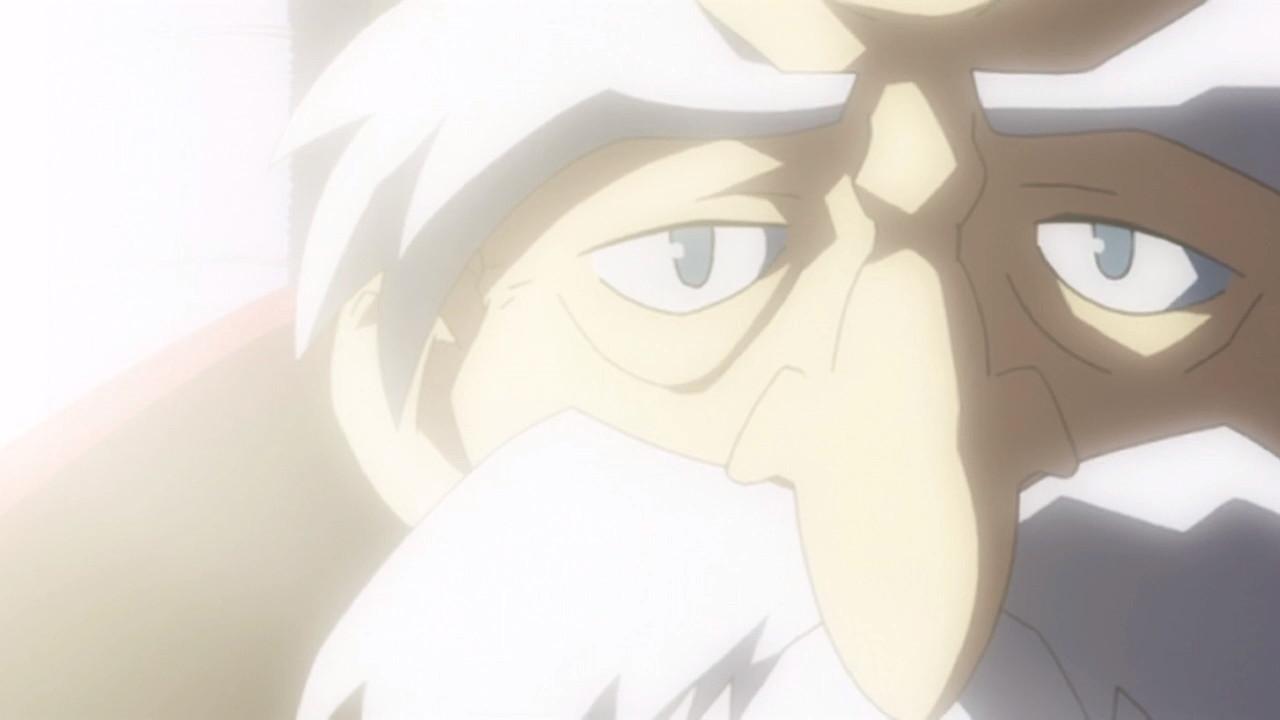
\includegraphics[width=0.5\linewidth]{figures/Characters/Char_Cain_MHX.jpg}
	\caption{Dr.~Cain as he appears in \emph{Day of $\Sigma$}.}
\end{figure}

Dr.~Cain is the brilliant scientist father of reploid's technology. Originally an archaeologist, Dr. Cain accidentally find Dr.~Light's laboratory while searching from prehistoric plant fossils, with X's capsules and blueprints inside~\cite{wiki:Cain_journal}-\cite{elysium_Cain_journal}, whom he befriends with. By using X's help, Dr.~Light's schematics and his knowledge of robotics, Dr. Cain manages to create his own version of a robots with free-will, which he label ``Reploids''. These new type robots greatly impacted on society, almost at the point of becoming necessary, in a very short amount of time and making Dr.~Cain one of the most important person of his world. However although Dr.~Cain's intention were surely good, aiming to achieve the same dream Dr.~Light had to create a society where humans and robots can life together, his actions were also the cause of firsts Maverick attacks~\cite{book:MH_field_guide}. In creating reploids, in fact, Cain didn't manage to fully recreate X's components, especially his ``Distress Circuit''~\cite{book:RMZ_Complete_works} and had to develop substitutes which where however prone to errors. Moreover these reploids' moral integrity wasn't tested for a period of time as long as X's one, making them more susceptible to taking a wrong path and going Maverick. Dr.~Cain seems partially to acknowledge his error, as after first mavericks appear he tries to find the cause of these problems\footnote{``\textit{This is the third instance of this type of behavior and I still have no idea of what is causing it!}'' - Journal of Dr.~Cain, $16^{th}$ July} develop more advanced reploids with more robust circuits to prevent errors, Sigma being the last of this series\footnote{``\textit{Sigma is one of the most intelligent reploids I've created and contains my latest circuit designs. His systems should be immune to any problems}'' - Journal of Dr.~Cain, $20^{th}$ November}. However even his latest designed circuits didn't manage to keep Sigma safe from going Maverick. Once Sigma begins his assault, Cain remains powerless to watch the destruction his creation caused believing nothing could stop him, not even X or Zero. However he doesn't either stop them from trying, as  he firmly believes something had to be done\footnote{``\textit{ I'm doubtful of their chances ( X and Zero), but I won't stop him. Something has to be done}'', Journal of Dr.~Cain, $4^{th}$ July}.

A different fate is instead reserved to Dr.~Cain's in the series remake, Maverick Hunter X. Here Cain's role remains the same up until Sigma's revolution, with the only difference of being much older and weaker, as he's connected to a life-support machine to extend his life for as much as he can. His only appearance is in the \emph{Day of $\Sigma$} OVA, where he explains to a pre-revolution Sigma the power X possesses and how it manifests in his hesitations and empathy, thus making Sigma interested in him. Cain is then seen only at the end of the OVA, after Sigma declares his war by launching missiles onto Abel city. He is last seen in his house, right before a missiles strikes directly onto it presumably killing him, pondering if reploids, created by humans but with abilities far beyond theirs, were fruit of mankind's arrogance rather than their good intentions and wish for knowledge\footnote{``\textit{Reploids... created by humanity, yet possessing abilities far beyond our own$\dots$ [$\dots$] Mankind's arrogance?$\dots$No}''-Dr.~Cain, Day of $\Sigma$, scene 4}.

%FROM HERE X2

\section{Serges} \label{char:Serges}
\begin{figure}[h]
	\centering
	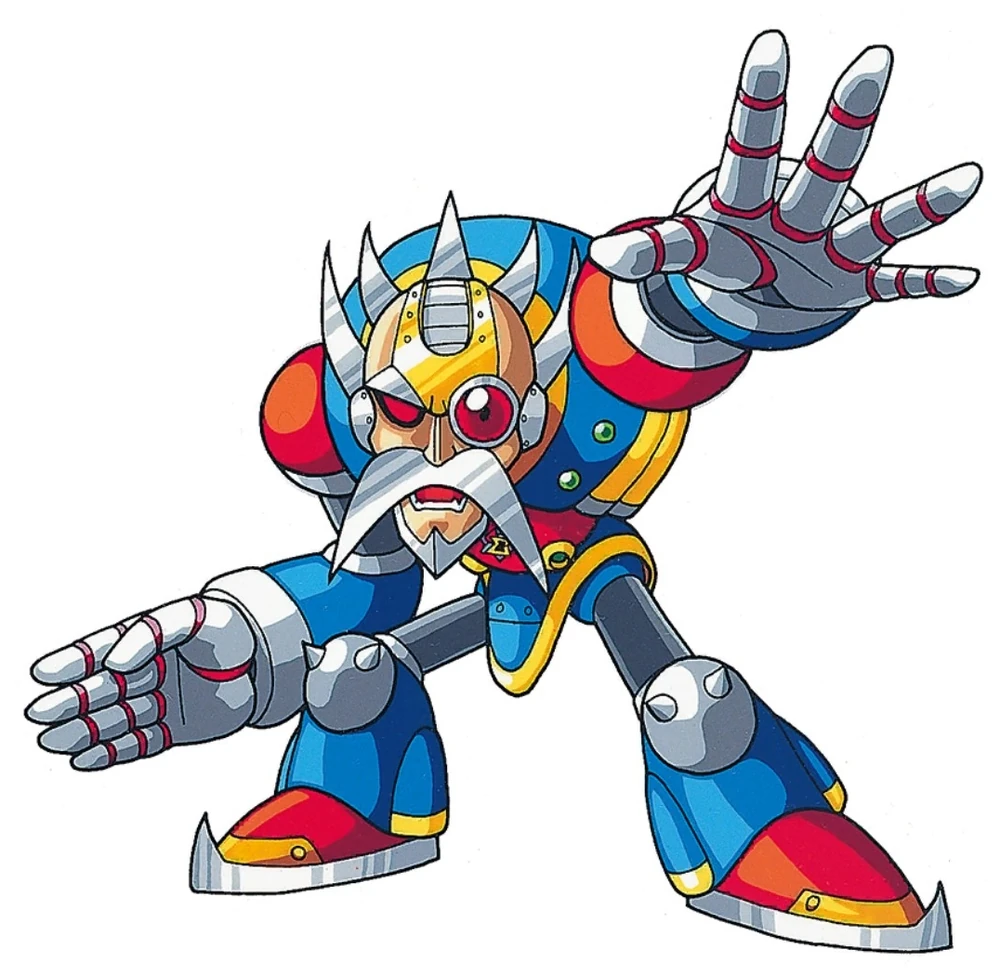
\includegraphics[width=0.4\linewidth]{figures/Characters/Char_Serges.png}
\end{figure}
Despite not playing a significant role in the game he appears in, Serges character and his links to other characters in the series have to be appointed and discussed. In particular what is worth to talk about are the possible connections that subsist between him and Dr.~Wily. By reading the original Japanese script for the X2 games and by studying also external sources (mainly listed in ~\cite{art:Serges_and_Isoc}) which talk about Serges it is, in fact, possible to draw a line which connect the
these two characters, albeit said connection has never been explicitly appointed. In these small sections the main evidences regarding this theory will be given.

The first possible connection between Serges and Wily comes from the original script for the X2 game. As, in fact, explained at the beginning of chapter~\ref{cha:X2}, the game underwent a massive localization causing an alteration in dialogues and the removal of some links in the finished product. In this context two are the main dialogues to focus on. The first one is the moment in which the X-Hunters contact X to challenge him in a fight. In the original script Serges opens his phrase by first calling X by his ``full'' name\footnote{\textit{Serges: … …crrrk… …bzzzt….Rock…E…cks…}- Serges,~\cite{wordpress:X2_japanese_script}} of \textit{Rockman X}, whereas no other character in the game addresses him in this way, Dr.~Cain included. The second, and probably most important, dialogue to be examined is Serge's final speech after being defeated the second time. In such occasion the original script report the following phrase:
\begin{quote}
	SERGES: Am I to perish here? Defeated by Light’s memento robot again… how regretful…~\cite{wordpress:X2_japanese_script}
\end{quote}
From these phrases Serges once again nods to the fact that he knows X and his origins more than any other. He not only, in fact, shows to know that X was built by Dr.~Light, information only Dr.~Cain knows, but also feeling regret for being defeated once more from a robot built by Light.  This feeling of regret, combined with the knowledge about X's past seems to point in the direction of Serges being, in some form, connected with Dr.~Wily, the original antagonist of the classic series.

Beside the original script, there is also other evidence which seems to point in this direction. According to the information given by the Rockman X2 Collected Sourcebook Information~\cite{wayback:X2_resources}, in fact, Serge's intellect surpasses even Sigma's and ties with Dr.~Wily's one. Furthermore from the same source it is possible to know that Serges was also responsible for the construction of Sigma's new body (a hard task considering the original Sigma was Dr.~Cain's best work) but more importantly for the rebuilding of Zero's body. Serges manages, in fact, not only to fully reconstruct Zero's body but also to upgrade it in its final form, such as by adding the shoulder pads, and also providing him with the signature Z-Saber. Beside the restoration, a task even Dr.~Cain refused to do due to how complicated Zero's design is\footnote{A truth which will hold up to X6 and beyond, where X and Zero's body will be considered a mystery}, it is the upgrade process the one on which to pause. Except for Zero's creator, in fact, no one would be able to know how to upgrade Zero or how he should look like once completed, especially since no one could know that Zero was unfinished in the first place. Since Zero's creator had been confirmed multiple times over various games, some more canon than others, to be Dr.~Wily (more details about this are given in chapter~\ref{char:Zero}), this strengthens even more the connection between Serges and Wily. In particular in the game Mega Man 2: The Power Fighters, in Bass' ending, a blueprint of Zero with his aspect from the X2 games onward appears, labeled as Dr.~Wily's new robot in development.  The theory of Serges and Wily being the same thing would also allow to explain how Sigma, in his final speech, acknowledge Zero's origins\footnote{\textit{But, Zero, why…he’s…the last of…Wi…num…ers…}-Sigma~\cite{wayback:X2_resources}}, which Sigma could not known if not for someone (such as Serges) had previously told him about.

It is however to underline that despite the evidence presented, the relationship between Serges and Wily is and will remain a mystery since, as stated in the Mega Man X Official Complete Works by Inafune himself, ``\textit{this is one of those things that is best left without an official comment}''~\cite{book:MMX_Complete_art}.
